% main.tex - Master Document
% כלי בינה מלאכותית בעסקים (AI Tools in Business)
% Authors: Dr. Yoram Segal & Prof. Eran Sheriff
% Compiler: LuaLaTeX
% CLS: hebrew-academic-template v5.11.0 (Book Class Support)

\documentclass[book]{hebrew-academic-template}

%% ============================================
%% Book-Specific Packages (not in CLS)
%% ============================================
\usepackage{tikz}
\usetikzlibrary{shapes,arrows,positioning,calc,fit,backgrounds,decorations.pathreplacing,mindmap,shadows}
\usepackage{pgfplots}
\pgfplotsset{compat=1.18}
\usepackage{multirow}
\usepackage{colortbl}
\usepackage{listings}

%% ============================================
%% Book Colors
%% ============================================
\definecolor{chaptercolor}{RGB}{0,51,102}
\definecolor{sectioncolor}{RGB}{0,76,153}
\definecolor{examplecolor}{RGB}{230,242,255}
\definecolor{exercisecolor}{RGB}{255,248,220}
\definecolor{codebackground}{RGB}{245,245,245}
\definecolor{formulacolor}{RGB}{240,255,240}

%% ============================================
%% Code Listings Configuration
%% ============================================
\lstset{
  basicstyle=\ttfamily\small,
  backgroundcolor=\color{codebackground},
  frame=single,
  breaklines=true,
  numbers=left,
  numberstyle=\tiny\color{gray},
  keywordstyle=\color{blue}\bfseries,
  commentstyle=\color{green!50!black},
  stringstyle=\color{red!60!black},
  showstringspaces=false,
  tabsize=4
}

\lstdefinestyle{python}{
  language=Python,
  morekeywords={self,True,False,None,as,with,async,await}
}

\lstdefinestyle{json}{
  basicstyle=\ttfamily\small,
  stringstyle=\color{red!60!black},
  morestring=[b]",
  literate=
    *{:}{{{\color{blue}:}}}{1}
    {,}{{{\color{blue},}}}{1}
    {\{}{{{\color{blue}\{}}}{1}
    {\}}{{{\color{blue}\}}}}{1}
    {[}{{{\color{blue}[}}}{1}
    {]}{{{\color{blue}]}}}{1}
}

%% ============================================
%% Bibliography
%% ============================================
\addbibresource{bibliography/references.bib}

%% ============================================
%% Additional Commands
%% ============================================
\newcommand{\term}[1]{\textbf{\textenglish{#1}}}
\newcommand{\heterm}[2]{\textbf{#1} (\textenglish{#2})}

\begin{document}

%% ============================================
%% Front Matter
%% ============================================
\frontmatter

%% Title Page
\begin{titlepage}
\begin{center}

\vspace*{2cm}

{\Huge\bfseries\color{chaptercolor} כלי בינה מלאכותית בעסקים}

\vspace{0.5cm}

{\Large\en{AI Tools in Business}}

\vspace{0.3cm}

{\large\en{(Agentic AI Engineering)}}

\vspace{2cm}

{\LARGE מאת}

\vspace{0.5cm}

{\Large\bfseries דר' יורם סגל}

\vspace{0.3cm}

{\Large ו}

\vspace{0.3cm}

{\Large\bfseries פרופסור ערן שריף}

\vspace{3cm}

\begin{english}
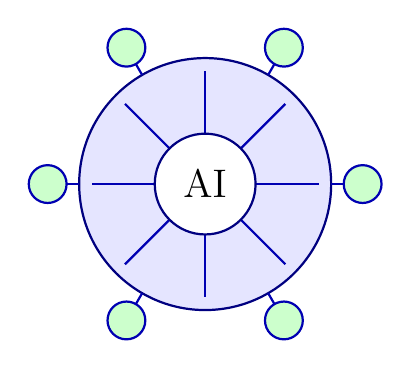
\begin{tikzpicture}[scale=0.8]
  % AI Brain Icon
  \draw[thick, blue!50!black, fill=blue!10] (0,0) circle (2cm);
  \foreach \i in {0,45,...,315} {
    \draw[thick, blue!70!black] (0,0) -- (\i:1.8);
  }
  \draw[thick, blue!50!black, fill=white] (0,0) circle (0.8cm);
  \node at (0,0) {\Large\textenglish{AI}};

  % Connection nodes
  \foreach \i in {0,60,...,300} {
    \draw[thick, blue!70!black, fill=green!20] (\i:2.5) circle (0.3cm);
    \draw[thick, blue!70!black] (\i:2) -- (\i:2.2);
  }
\end{tikzpicture}
\end{english}

\vspace{2cm}

{\large ספר לימוד לתואר שני במנהל עסקים}

\vspace{0.5cm}

{\normalsize מהדורה ראשונה -- \en{2025}}

\vfill

{\small כל הזכויות שמורות לדר' יורם סגל ופרופסור ערן שריף}

\end{center}
\end{titlepage}

%% Copyright Page
\newpage
\thispagestyle{empty}
\vspace*{\fill}
\begin{center}
{\small
כל הזכויות שמורות \en{© 2025}

דר' יורם סגל ופרופסור ערן שריף

\vspace{1cm}

אין לשכפל, להעתיק, לצלם, להקליט, לתרגם, לאחסן במאגר מידע,
לשדר או לקלוט בכל דרך או בכל אמצעי אלקטרוני, אופטי או מכני
או אחר -- כל חלק שהוא מהחומר שבספר זה.

שימוש מסחרי מכל סוג שהוא בחומר הכלול בספר זה אסור בהחלט,
אלא ברשות מפורשת בכתב מהמחברים.

\vspace{1cm}

\en{All rights reserved © 2025}

\en{Dr. Yoram Segal \& Prof. Eran Sheriff}
}
\end{center}
\vspace*{\fill}

%% Table of Contents
\tableofcontents

%% List of Figures
\listoffigures

%% List of Tables
\listoftables

%% Preface
\chapter*{הקדמה}
\addcontentsline{toc}{chapter}{הקדמה}

ברוכים הבאים לספר "כלי בינה מלאכותית בעסקים".

אנו חיים בעידן של מהפכה טכנולוגית חסרת תקדים. מודלי שפה גדולים (\en{LLMs}) ובינה מלאכותית יוצרת משנים את האופן שבו עסקים פועלים, מקבלים החלטות ומתקשרים עם לקוחותיהם. כמנהלים בעידן הזה, ההבנה של הכלים הללו אינה עוד מותרות -- היא הכרח.

ספר זה נכתב עבור מנהלים ברמת \en{MBA} שרוצים להבין את עולם ה-\en{AI} העסקי לעומק, אך ללא הצורך להפוך למהנדסי תוכנה. המטרה שלנו היא לספק לכם את הידע הדרוש לקבלת החלטות מושכלות, לתכנון אסטרטגי של הטמעת \en{AI} בארגון, ולהובלת פרויקטים בתחום.

הספר מחולק ל-\en{13} פרקים, פרק לכל שבוע בסמסטר. כל פרק בנוי על קודמיו, ויחד הם יוצרים תמונה שלמה של האקוסיסטם של \en{AI} בעסקים -- מהיסודות התיאורטיים ועד ליישום מעשי מקצה לקצה.

בכל פרק תמצאו:
\begin{itemize}
  \item הסברים תיאורטיים בסגנון נגיש וסיפורי
  \item נוסחאות מנהליות לחישוב \en{ROI}, עלויות והחזר השקעה
  \item תרשימים וגרפים להמחשה ויזואלית
  \item דוגמאות מעשיות מעולם העסקים
  \item תרגילים תיאורטיים ומעשיים עם פתרונות
  \item קוד \en{Python} להתנסות מעשית
\end{itemize}

אנו מאחלים לכם למידה פורייה ומהנה.

\vspace{1cm}

\begin{flushright}
דר' יורם סגל ופרופסור ערן שריף

\en{2025}
\end{flushright}

%% ============================================
%% Main Matter
%% ============================================
\mainmatter

% Chapter 1: Introduction to LLMs
\subfile{chapters/chapter-01}

% Chapter 2: AI Ecosystem
\subfile{chapters/chapter-02}

% Chapter 3: REST APIs and JSON
\subfile{chapters/chapter-03}

% Chapter 4: MCP Protocol
\subfile{chapters/chapter-04}

% Chapter 5: Autonomous Agents
\subfile{chapters/chapter-05}

% Chapter 6: A2A Protocol
\subfile{chapters/chapter-06}

% Chapter 7: RAG Systems
\subfile{chapters/chapter-07}

% Chapter 8: Prompt Engineering
\subfile{chapters/chapter-08}

% Chapter 9: Deployment
\subfile{chapters/chapter-09}

% Chapter 10: Strategic Considerations
\subfile{chapters/chapter-10}

% Chapter 11: Interfaces and UX
\subfile{chapters/chapter-11}

% Chapter 12: Ethics, Regulation and Security
\subfile{chapters/chapter-12}

% Chapter 13: From Project to Product
\subfile{chapters/chapter-13}

%% ============================================
%% Back Matter
%% ============================================
\backmatter

%% Bibliography - IEEE format LTR
\begingroup
\begin{english}
\pardir TLT
\printbibliography[heading=bibintoc,title={References / \texthebrew{רשימת מקורות}}]
\end{english}
\endgroup

%% Appendices
\appendix

\hebrewappendix{מילון מונחים}

\begin{longtable}{p{4cm}p{4cm}p{6cm}}
\toprule
\textbf{מונח באנגלית} & \textbf{תרגום לעברית} & \textbf{הסבר} \\
\midrule
\endhead

\en{LLM} & \hebcell{מודל שפה גדול} & \hebcell{מודל בינה מלאכותית המאומן על כמויות עצומות של טקסט} \\
\en{API} & \hebcell{ממשק תכנות יישומים} & \hebcell{דרך סטנדרטית לתקשורת בין מערכות} \\
\en{REST} & \hebcell{העברת מצב ייצוגי} & \hebcell{ארכיטקטורת תקשורת נפוצה ל-\en{API}} \\
\en{JSON} & \hebcell{סימון אובייקט \en{JavaScript}} & \hebcell{פורמט להעברת נתונים} \\
\en{MCP} & \hebcell{פרוטוקול הקשר מודל} & \hebcell{פרוטוקול להעברת הקשר למודלי \en{AI}} \\
\en{Agent} & \hebcell{סוכן} & \hebcell{תוכנה אוטונומית המבצעת משימות} \\
\en{A2A} & \hebcell{סוכן-לסוכן} & \hebcell{תקשורת בין סוכנים אוטונומיים} \\
\en{RAG} & \hebcell{יצירה מועשרת באחזור} & \hebcell{טכניקה לשילוב ידע עדכני ב-\en{LLM}} \\
\en{Prompt} & \hebcell{פרומפט/הנחיה} & \hebcell{הטקסט שנשלח ל-\en{LLM} לעיבוד} \\
\en{Token} & \hebcell{טוקן} & \hebcell{יחידת עיבוד בסיסית של \en{LLM}} \\
\en{Embedding} & \hebcell{שיבוץ/הטמעה} & \hebcell{ייצוג וקטורי של טקסט} \\
\en{Vector Database} & \hebcell{בסיס נתונים וקטורי} & \hebcell{מאגר לאחסון וחיפוש וקטורים} \\
\en{Fine-tuning} & \hebcell{כוונון עדין} & \hebcell{התאמת מודל קיים לתחום ספציפי} \\
\en{Hallucination} & \hebcell{הזיה} & \hebcell{יצירת מידע שגוי על ידי \en{LLM}} \\
\en{Context Window} & \hebcell{חלון הקשר} & \hebcell{כמות הטקסט שהמודל יכול לעבד בבת אחת} \\
\bottomrule
\end{longtable}

\hebrewappendix{קוד \en{Python} מלא}

פרק זה מכיל את כל קטעי הקוד המופיעים בספר במלואם, מוכנים להעתקה והרצה.

% Code snippets will be included here

\end{document}
